\subsection{Rozszerzone sieci przejść}
Biorąc pod uwagę gramatykę predykatową \(G = (N, T, P, S, \Pi, \mathcal{M})\)
odpowiedni ATN \(M_G = (Q, \Sigma, \Delta, E, F) \) ma elementy [20]: 
\begin{itemize}
\item Q jest zbiorem stanów
\item \( \Sigma \) jest alfabetem krawędzi \( N \cup T \cup  \Pi \cup \mathcal{M}\)
\item \( \Delta \) relacją przejść mapującą \( Q \times (\Sigma \cup \epsilon) \rightarrow Q \) 
\item \( E \subset Q = \{p_A|A \in N\} \) jest zbiorem stanów początkowych subautomatu
\item \( F \subset Q = \{p'_A|A \in N\} \) jest zbiorem stanów końcowych subautomatu
\end{itemize}

\begin{figure}[h]
\begin{tabular}{c|c} 
  \hline
  \head{Element gramatyki wejściowej} & \head{Wynikowe przejścia ATN} \\
  \hline
  \(A \rightarrow \alpha_i \) & \(p_A \overset{\epsilon}{\rightarrow} p_{A,i}
                  \overset{\epsilon}{\rightarrow} \boxed{\alpha_i} \overset{\epsilon}{\rightarrow} p'_A \) \\
  \(A \rightarrow \{ \pi_i \}? \alpha_i \) & \(p_A \overset{\epsilon}{\rightarrow} p_{A,i}
                  \overset{\pi_i}{\rightarrow} \boxed{\alpha_i} \overset{\epsilon}{\rightarrow} p'_A \) \\
  \(A \rightarrow \{ \mu_i \}  \) & \(p_A \overset{\epsilon}{\rightarrow} p_{A,i}
                  \overset{\mu_i}{\rightarrow} p'_A \) \\
  \(A \rightarrow  \epsilon_i \) & \(p_A \overset{\epsilon}{\rightarrow} p_{A,i}
                  \overset{\epsilon}{\rightarrow} p'_A \) \\
  \( \boxed{\alpha_i} = X_1X_2...X_m \) \\ for \( X_j \in N \cup T \),j=1..m  & \( p_0
                  \overset{X_1}{\rightarrow} p_1 \overset{X_2}{\rightarrow} ... \overset{X_m}{\rightarrow} p_m \) \\
  \hline
\end{tabular}
\caption{Transformacja gramatyki predykatowej do ATN}
\end{figure}

\begin{figure}[h]
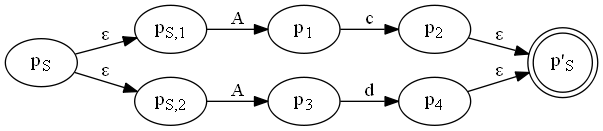
\includegraphics[width=0.45\textwidth]{Figure8a.png}
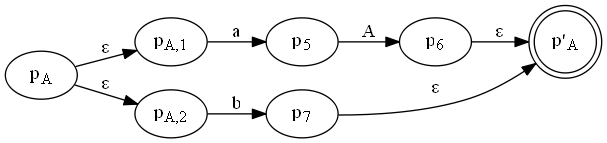
\includegraphics[width=0.45\textwidth]{Figure8b.png}
\caption{ATN dla G z \( P = \{S \rightarrow Ac|Ad, A \rightarrow aA|b \} \)}
\end{figure}

ATNy przypominają diagramy składni, używane do dokumentowania języków programowania,
z podautomatami ATN dla poszczególnych symboli nieterminalnych.
Rysunek 7 przedstawia jak utworzyć zbiór stanów Q i krawędzie \( \Delta \)
z produkcji gramatyki. Początkowy stan dla A jest \( p_A \in Q \)
i jest skierowany na \( p_{A,i} \) utworzony z lewej strony krawędzi \( \alpha_i \) ,
z krawędzią w \( \Delta \). Ostatni stan utworzony z \( \alpha_i \) jest skierowany na \( p'_A \).
Nieterminalne krawędzie \( p \overset{A}{\rightarrow} q\) są niczym wywołania funkcji.
Przenoszą kontrolę ATN na podautomat A, wkładając stan powrotny q na stos wywołań,
tak aby mógł kontynuować z q po osiągnięciu stanu stop dla A podautomatu \( p'_A \).
Rysunek 8 przedstawia ATN dla prostej gramatyki.
Język rozpoznawany przez ATN jest taki sam, jak oryginalny język gramatyczny.
